
\documentclass{beamer}

\usepackage[utf8]{inputenc}
\usetheme{Madrid}
\usecolortheme{default}

%Information to be included in the title page:
\title[PaperSharing-(EACL'21)LTR]{[EACL'21] On the Calibration and Uncertainty of Neural Learning to Rank Models}
\author[Shengqiang Zhang]{Gustavo Penha \and Claudia Hauff}
\institute[Baidu]{Delft University of Technology, Delft, Netherlands}
\date{2021.1.25}

\AtBeginSection[]
{
  \begin{frame}
    \frametitle{Table of Contents}
    \tableofcontents[currentsection]
  \end{frame}
}

\begin{document}

\frame{\titlepage}

\begin{frame}
\frametitle{Table of Contents}
\tableofcontents
\end{frame}

\section{Motivation}
\begin{frame}{Motivation}
    \begin{block}{Probability Ranking Principle(PRP) (Robertson, 1977)}
    ranking documents in decreasing order of their probability of relevance leads to an optimal document ranking for ad-hoc retrieval.
    \end{block}
    
    For the PNP to hold, ranking models must at least meet the following conditions (Gordan and Lenk, 1991):
    \begin{itemize}
        \item [C1] assign \textbf{well calibrated} probabilities of relevance, i.e. if we gather all documents for which the model predicts relevance with a probability of e.g. 30\%, the amount of relevant documents should be 30\%
        \item [C2] the probabilities of relevance are reported \textbf{with certainty}
    \end{itemize}
    
\end{frame}

\begin{frame}{Motivation}
\begin{itemize}
    \item [C1] It has been shown that DNNs are not well calibrated in the context of computer vision (Guo et al., 2017).
    \item [C2] There are a number of sources of uncertainty in the training process of neural networks that make it unreasonable to assume that neural ranking models fulfill [C2]: 
    \begin{itemize}
        \item \textsl{parameter uncertainty}
        \item \textsl{structural uncertainty}
        \item \textsl{aleatoric uncertainty}
    \end{itemize}
    Given these sources of uncertainty, using point estimate predictions and ranking according to the PRP might not achieve the optimal ranking for retrieval.
\end{itemize}
\end{frame}

\begin{frame}{What's Next?}
\begin{enumerate}
    \item Analyze the calibration of neural rankers, specially BERT-based rankers.
    \item To model the uncertainty of BERT-based rankers, we propose \textsl{stochastic neural ranking models} by applying different techniques to model uncertainty of DNNs:
        \begin{itemize}
            \item MC Dropout
            \item Deep Ensembles
        \end{itemize}
\end{enumerate}
\end{frame}


\section{Background and Related Work}
\begin{frame}{Calibration and Uncertainty in IR}
\begin{enumerate}
    \item Calibration: 
        \begin{itemize}
            \item The calibration of ranking models has received little attention in IR.
            \item Important in automated medical domain due to model interpretability
        \end{itemize}
    \item Uncertainty: 
        \begin{itemize}
            \item Treating \textbf{variance} as a measure of uncertainty inspired by economics theory.
            \item Applications:
                \begin{itemize}
                    \item improve the ranking effectiveness
                    \item in conversational search, decide between asking clarifying questions and providing a potential answer
                    \item perform dynamic query reformulation for queries where the intent is uncertain
                    \item predict answers with no correct answers
                \end{itemize}
        \end{itemize}
\end{enumerate}
    
\end{frame}

\section{Model}
\begin{frame}{Research Questions}
We introduce the models for answering the following research questions:
\begin{itemize}
    \item [RQ1] How calibrated are deterministic and stochastic BERT-based rankers?
    \item [RQ2] Are the uncertainty estimates from stochastic BERT-based rankers useful for risk-aware ranking?
    \item [RQ3] Are the uncertainty estimates obtained from stochastic BERT-based rankers useful for identifying unanswerable queries?
\end{itemize}
\end{frame}

\begin{frame}{Measuring Calibration(RQ1)}
\begin{block}{Empicical Calibration Error(ECE)}
ECE is an intuitive way of measuring to what extent the confidence scores
from neural networks align with the true correctness likelihood. It measures the difference between the observed reliability curve (DeGroot and Fienberg, 1983) and the ideal one.
\end{block}
We sort the predictions of the model, divide them into $c$ buckets $\{B_0, ..., B_c\}$, and take the weighted average
between the average predicted probability
of relevance $avg(B_i)$ and the fraction of relevant
documents $\frac{rel(B_i)}{|B_i|}$ in the bucket:
\begin{equation}
    ECE = \sum_{i=0}^c \frac{|B_i|}{n} \left|avg(B_i) - \frac{rel(B_i)}{|B_i|} \right|
\end{equation}
where n is the total number of test examples.
\end{frame}

\begin{frame}{Modeling Uncertainty}
\begin{enumerate}
    \item Define the ranking problem we focus on
    \item Deterministic BERT-based ranker baseline model(\textbf{BERT})
    \item Our model to answer RQ2 and RQ3:
        \begin{itemize}
            \item a stochatic BERT-based ranker to model uncertainty(\textbf{S-BERT})
            \item a risk-aware BERT-based ranker to take into account uncertainty provided by S-BERT when ranking(\textbf{RA-BERT})
        \end{itemize}
\end{enumerate}
\end{frame}

\begin{frame}{Conversation Response Ranking}
Let $\mathcal{D} = \{(\mathcal{U}_i, \mathcal{R}_i, \mathcal{Y}_i) \}_{i=1}^N $ be a dataset consisting of N triplets: dialogue context, response candidates and response relevance labels.
\begin{itemize}
    \item $\mathcal{U}_i = \{u^1, u^2, ..., u^{\tau}\}$
    \item $\mathcal{R}_i = \{r^1, r^2, ..., r^K \}$
    \item $\mathcal{Y}_i = \{y^1, y^2, ..., y^k \}$
\end{itemize}
The task is to learn a ranking function $f(.)$ that is able to generate a
ranked list for the set of candidate responses $\mathcal{R}_i$
based on their predicted relevance scores $f(\mathcal{U}_i, r)$
\end{frame}

\begin{frame}{Deterministic BERT Ranker}
Pointwise BERT
    
\end{frame}

\begin{frame}{Stochastic S-BERT Ranker}
We want to obtain a predictive distribution which allows us to extract uncertainty estimates
\begin{equation}
    R_r = \{ f(\mathcal{U}_i, r)^0, f(\mathcal{U}_i, r)^1, ..., f(\mathcal{U}_i, r)^n \}
\end{equation}

\begin{columns}

\column{0.5\textwidth}
Two techniques:
\begin{enumerate}
    \item Deep Ensembles($\textbf{S-BERT}^\textbf{E}$)
    \item MC Dropout($\textbf{S-BERT}^\textbf{D}$)
\end{enumerate}

\column{0.5\textwidth}
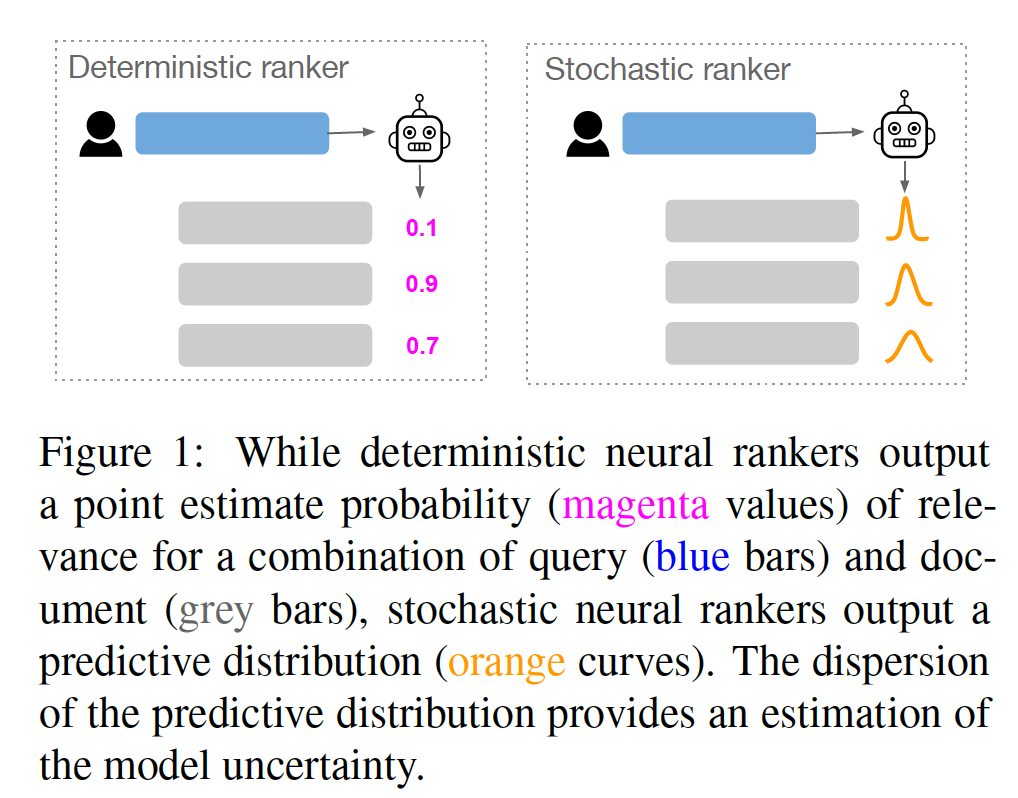
\includegraphics[scale=0.3]{figure1.png}
\end{columns}

\end{frame}

\begin{frame}{Deep Ensembles(\textbf{S-BERT}^{\textbf{E}})}
We train $M$ models using different random seeds and make predictions with each one of them to generate M predicted values:
\begin{equation}
    R^{E}_{r} = \{ f(\mathcal{U}_i, r)^0, f(\mathcal{U}_i, r)^1, ..., f(\mathcal{U}_i, r)^M \}
\end{equation}
The mean of the predicted values is used as the predicted probability of relevance:
\begin{equation}
    \textbf{S-BERT}^{\textbf{E}}(\mathcal{U}_i, r) = E[R^E_r]
\end{equation}
The variance $var[R^E_r]$ gives us a measure of the uncertainty in the prediction.
\end{frame}

\begin{frame}{MC Dropout(\textbf{S-BERT}^{\textbf{D}})}
We train a single model and employ dropout at test time and generate stochastic predictions of relevance by conducting T forward passes:
\begin{equation}
    R^{D}_{r} = \{ f(\mathcal{U}_i, r)^0, f(\mathcal{U}_i, r)^1, ..., f(\mathcal{U}_i, r)^T \}
\end{equation}
The mean of the predicted values is used as the predicted probability of relevance:
\begin{equation}
    \textbf{S-BERT}^{\textbf{D}}(\mathcal{U}_i, r) = E[R^D_r]
\end{equation}
The variance $var[R^D_r]$ gives us a measure of the uncertainty in the prediction.

\end{frame}

\begin{frame}{Risk-Aware RA-BERT Ranker}
    Given the predictive distribution $R_r$, obtained either by \textbf{Ensemble} or \textbf{Dropout}, we use the following function to rank responses with riskawareness:
    \begin{equation}
        \textbf{RA-BERT}(\mathcal{U}_i, r) = E[R_r] - b * var[R_r] - 2b\sum_i^{n-1}cov[R_r, R_{r_i}]
    \end{equation}
    where b is a hyperparameter that controls the aversion or predilectioin towards risk.
    
    \begin{itemize}
        \item $\textbf{RA-BERT}^\textbf{D} $ when using $\textbf{S-BERT}^\textbf{D}$'s predictive distribution
        \item $\textbf{RA-BERT}^\textbf{E} $ when using $\textbf{S-BERT}^\textbf{D}$'s predictive distribution
    \end{itemize}
\end{frame}

\begin{frame}{Robustness to Distributional Shift}
In order to evaluate whether we can trust the model’s calibration and uncertainty estimates, we evaluate how robust the models are to different types of shift in the test data.

For all three research questions, we test the models under the following two settings:
\begin{enumerate}
    \item Cross Domain
    \item Cross Negative Sampling: test models on negative documents that were sampled using a different NS strategy than during training.
        \begin{itemize}
            \item $\textbf{NS}_{random}$
            \item $\textbf{NS}_{classic}$
            \item $\textbf{NS}_{sentenceEmb}$
        \end{itemize}
        
\end{enumerate}
    
\end{frame}

\section{Experiments}
\begin{frame}{Experimental Setup}
\begin{enumerate}
    \item Dataset
        \begin{itemize}
            \item MSDialog (246k context-response pairs, from the MS QA forum for several Microsoft products)
            \item MANTis (1.3 million context-response pairs, from 14 Stack Exchange sites, such as \textsl{askubuntu} and \textsl{travel}
            \item $UDC_{DSTC8}$ (184k context-response pairs of disentangled Ubuntu IRC dialogues)
        \end{itemize}
    \item Implementation Details
        \begin{itemize}
            \item Training BERT using sample method of BM25
            \item $\textbf{NS}_{sentenceEmb}$ use \textbf{sentenceBERT} (Reimers and Gurevych, 2019)
            \item The baseline BERT-based ranker setup yields comparable effectiveness with SOTA methods
        \end{itemize}
    \item Evaluation
        \begin{itemize}
            \item effectiveness: recall at positiion K with n candidates: $R_n@K$
            \item evaluate quality of the uncertainty estimation with two downstream tasks:
                \begin{itemize}
                    \item improve conversation response ranking itself via Risk-Aware ranking
                    \item predict unanswerable conversational contexts
                \end{itemize}
        \end{itemize}
\end{enumerate}
    
\end{frame}

\begin{frame}{Results: Calibration of Neural Rankers(RQ1)}
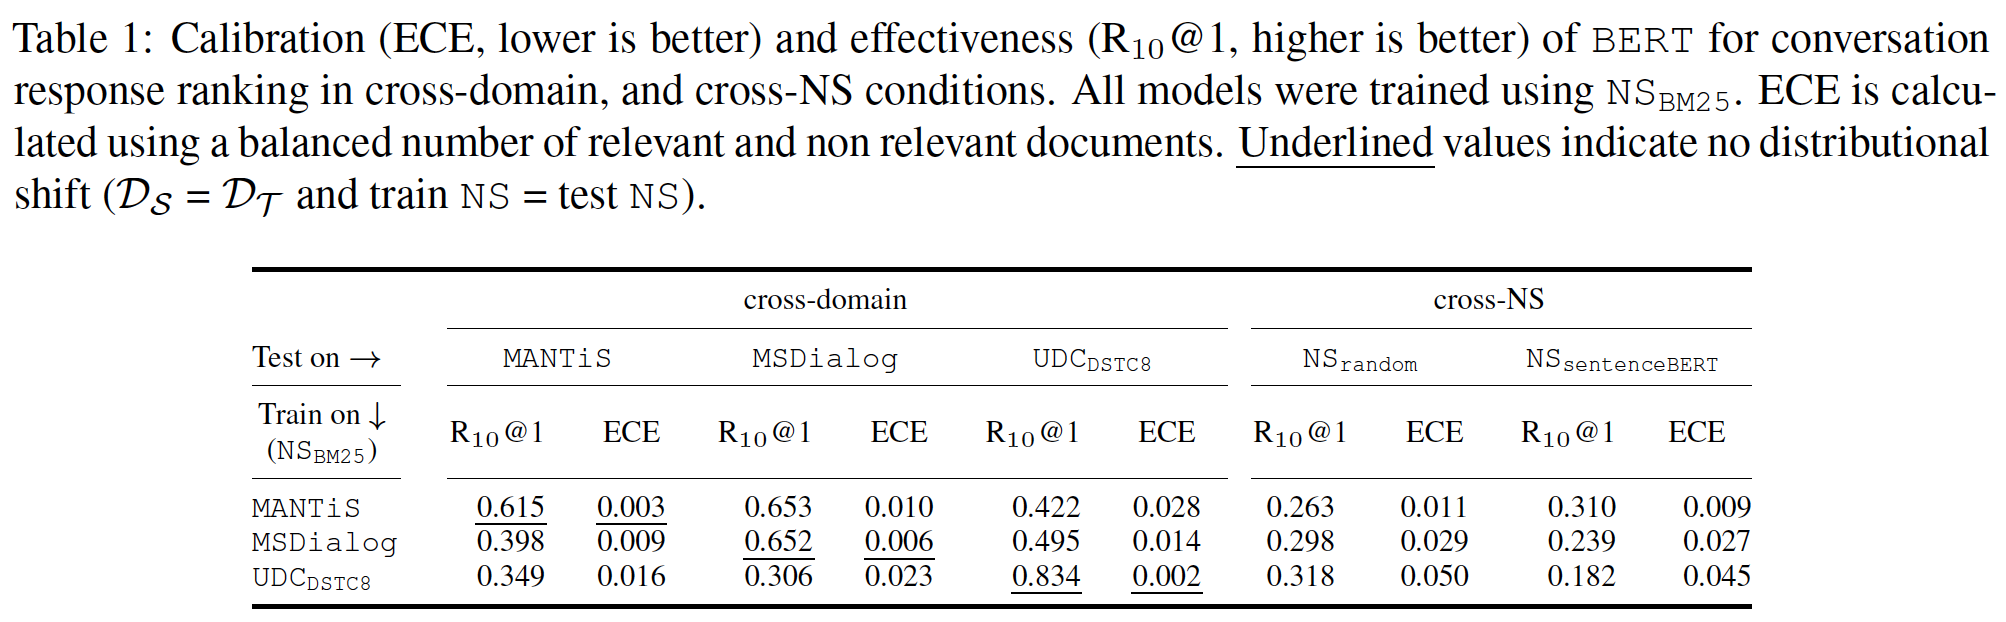
\includegraphics[scale=0.35]{table1.png}
\begin{itemize}
    \item \textbf{BERT} is both effective and calibrated under no distributional shift conditions. However, the calibration error increases significantly in cross-domain and cross-NS settings, \textbf{indicating that they do not have robust calibrated predictions}.
\end{itemize}
    
\end{frame}

\begin{frame}{Results: Calibration of Neural Rankers(RQ1)}
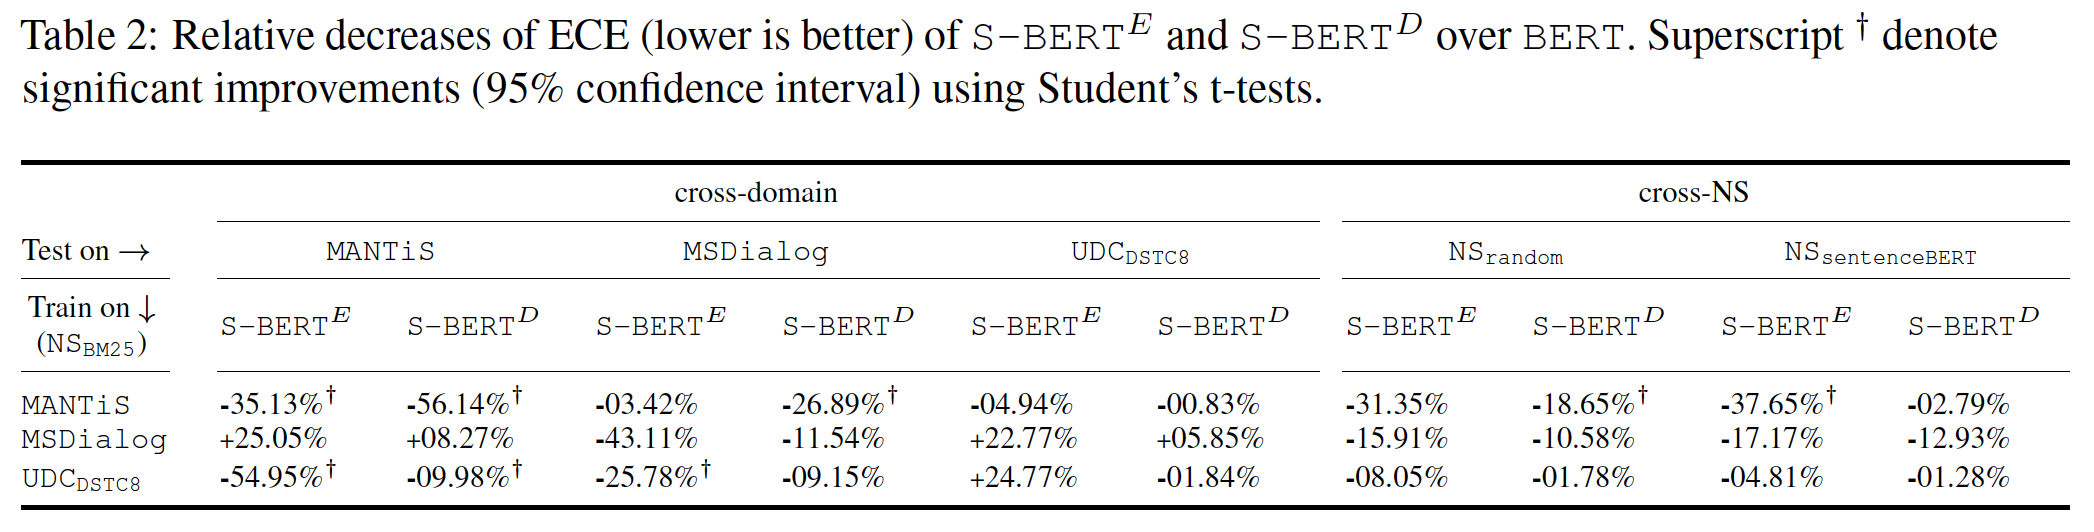
\includegraphics[scale=0.33]{table2.png}
\begin{itemize}
    \item \textbf{stochastic BERT} displays the improvements (relative drop in ECE) over \textbf{BERT} in terms of calibration.
    \item $\textbf{S-BERT}^{E}$ is on average \textbf{14\%} better than \textbf{BERT}, while $\textbf{S-BERT}^{D}$ is on average \textbf{10\%} better than \textbf{BERT}.
    \item \textbf{answering our RQ1: stochastic BERT-based rankers have better calibration than deterministic BERT-based ranker}
\end{itemize}
\end{frame}

\begin{frame}{Results: Uncertainty Estimates for Risk-Aware Neural Ranking(RQ2)}
    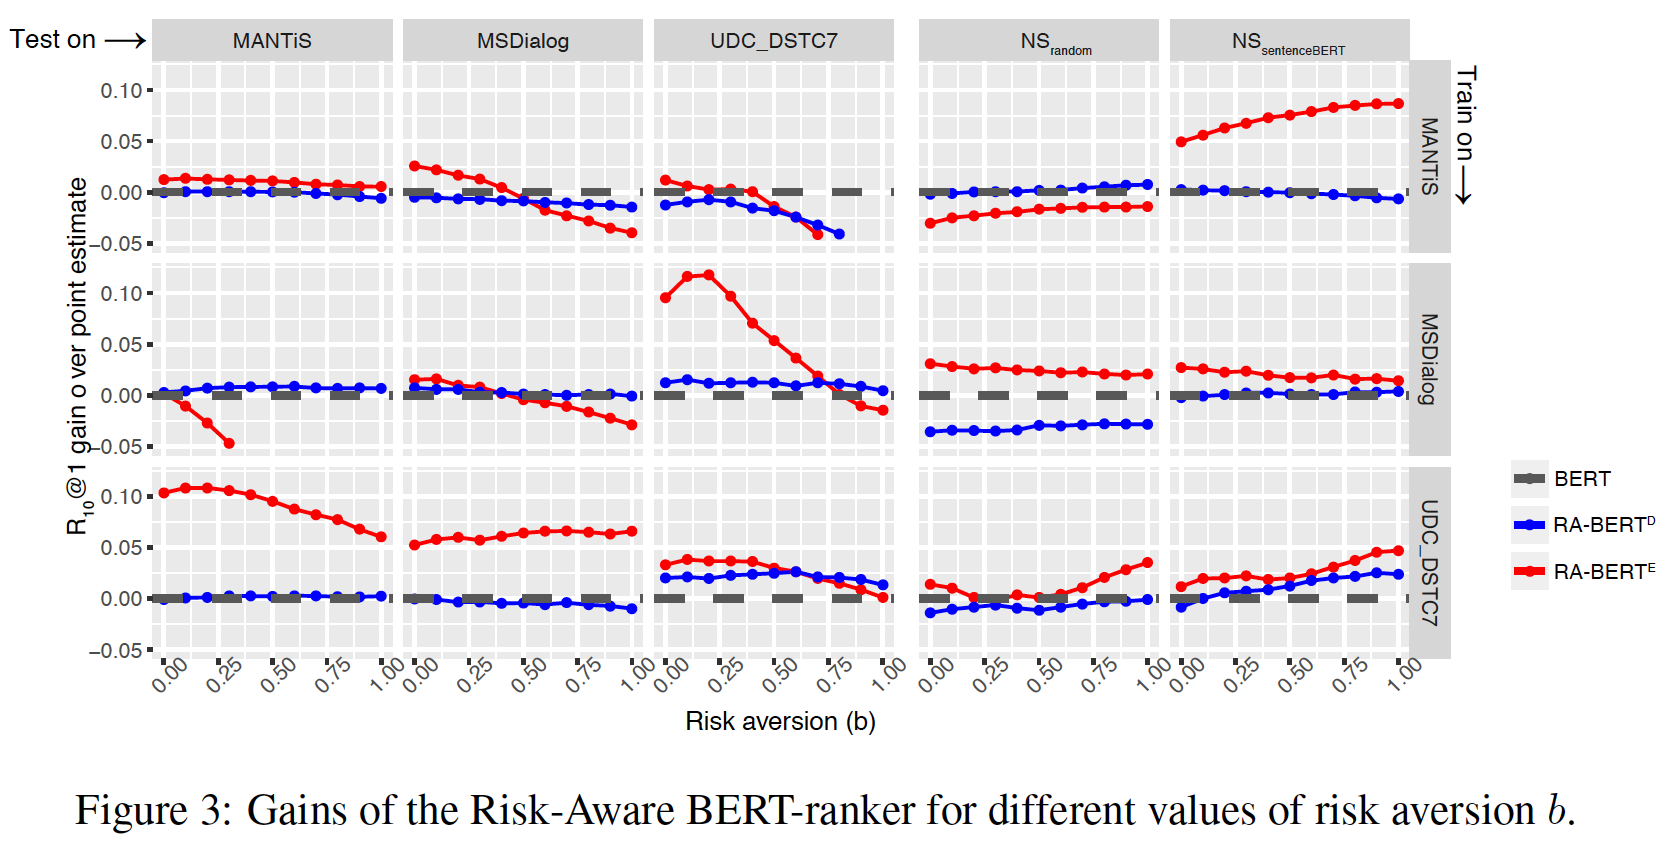
\includegraphics[scale=0.4]{figure3.png}
    
\end{frame}
\begin{frame}{Results: Uncertainty Estimates for Risk-Aware Neural Ranking(RQ2)}
    
    \begin{itemize}
        \item When $b = 0$, we are using the mean of the predictive distribution and disregard the risk, which is relevant to \textbf{S-BERT}
        \item When $b < 0$, we are ranking with risk predilection. In all conditions the effectiveness was significantly worse than when $b = 0$
        \item When increasing the risk aversion ($b > 0$), it has different effects depending on the combination of domain and NS.
    \end{itemize}
\end{frame}

\begin{frame}{Results: Uncertainty Estimates for Risk-Aware Neural Ranking(RQ2)}
In order to investigate whether ranking with risk aversion is more effective than using the predictive distribution mean, we select $b$ based on the best value observed on the validation set.

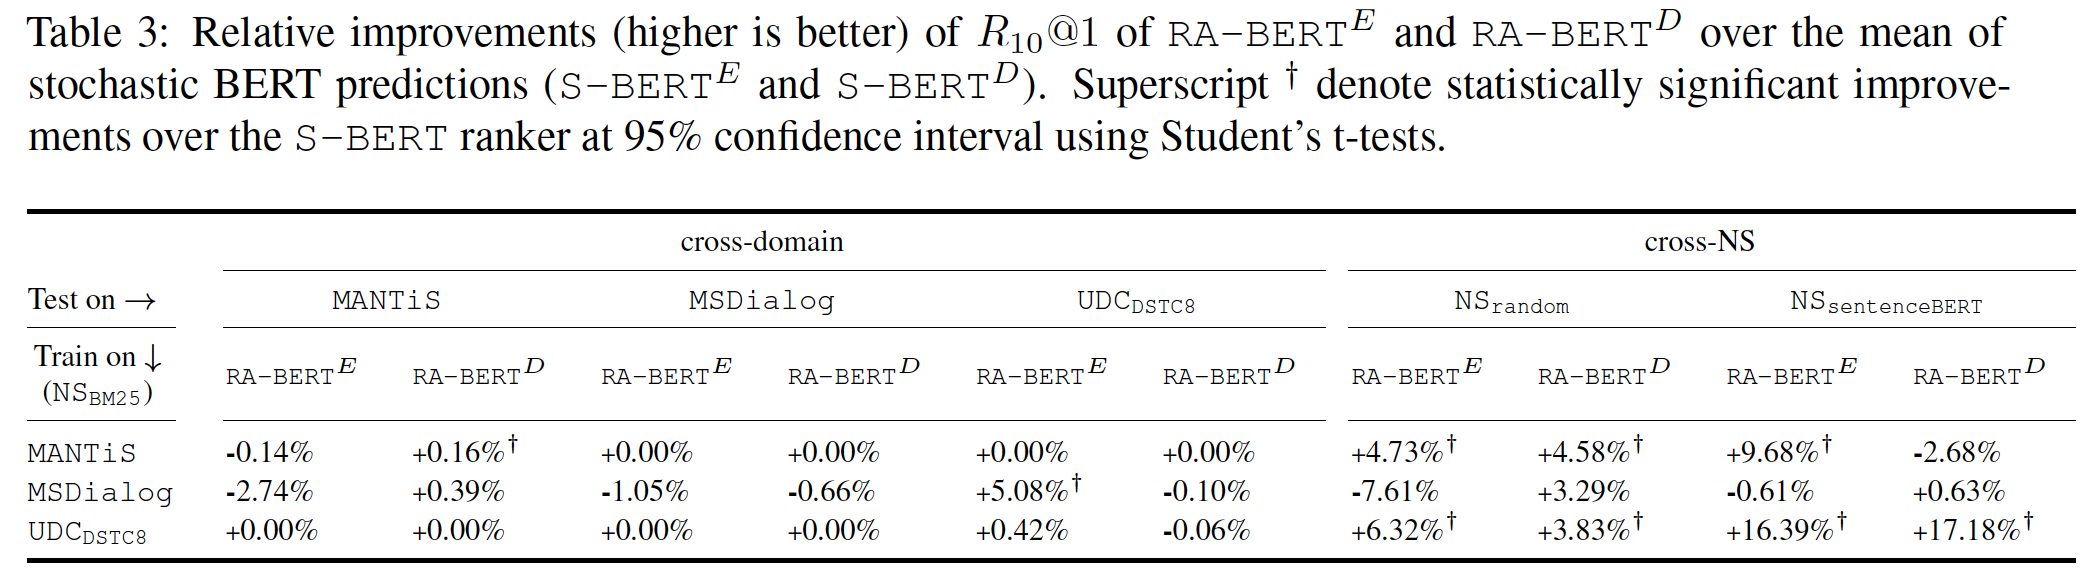
\includegraphics[scale=0.33]{table3.png}
\textbf{This answers our RQ2, indicating that the uncertainties obtained from stochastic neural rankers are useful for risk-aware ranking, specially in the cross-NS setting where the baseline model is quite ineffective.}
\end{frame}

\begin{frame}{Results: Uncertainty Estimates for NOTA prediction(RQ3)}
    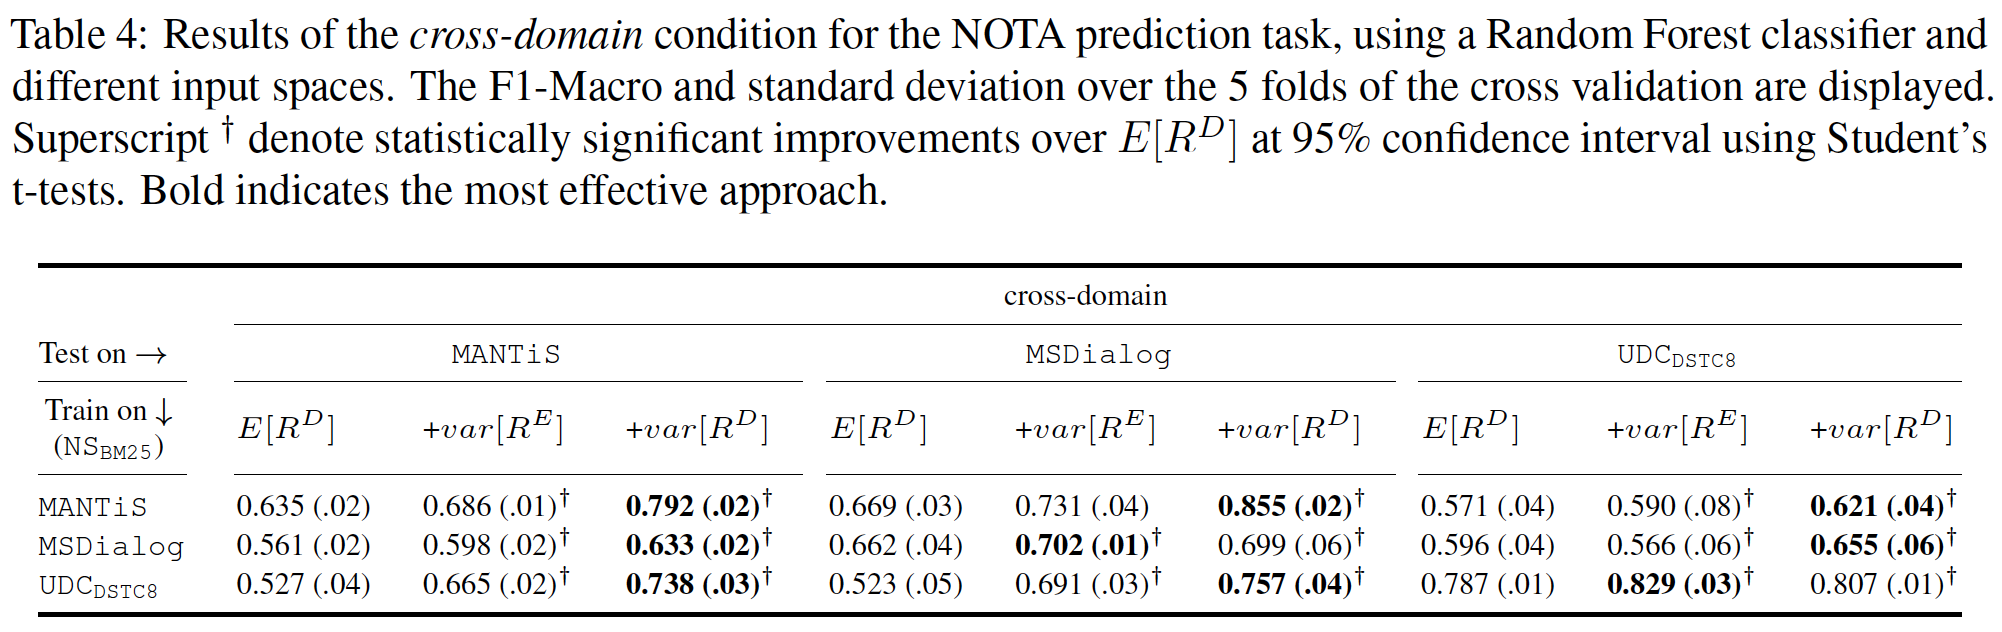
\includegraphics[scale=0.35]{table4.png}
    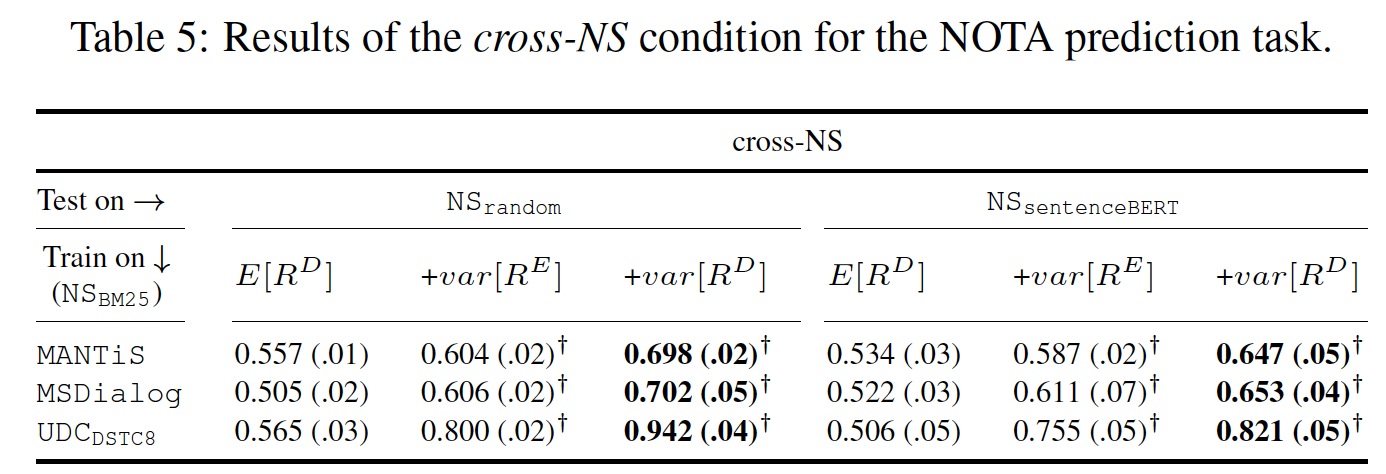
\includegraphics[scale=0.4]{table5.png}
\end{frame}

\begin{frame}{Results: Uncertainty Estimates for NOTA prediction(RQ3)}
The uncertainties from $\textbf{S-BERT}^D$ and $\textbf{S-BERT}^E$ significantly improve the F1 for NOTA prediction for both cross-domain and cross-NS settings
\begin{itemize}
    \item cross-domain: improvement of 24\% on average
    \item cross-NS: improvement of 46\% on average
\end{itemize}

\textbf{This answers our RQ3 that the uncertainty estimates from stochastic neural rankers do improve the effectiveness of the NOTA prediction task (by an average of 33\% for all conditions considered)}
\end{frame}
\section{Conclusion}
\begin{frame}{Conclusion}
\begin{enumerate}
    \item Show that deterministic BERT-based ranker is not robustly calibrated for the task of conversation response ranking
    \item Improve BERT-based ranker with two techniques to estimate uncertainty through \textsl{stochastic neural ranking}
    \item Benefits of estimating uncertainty using risk-aware neural ranking and for predicting unanswerable conversational contexts
\end{enumerate}
\end{frame}
\bibliography{references}
\bibliographystyle{acl_natbib}
\end{document}